\section{Current Results}
Gate F selected an oracle-analysis pivot. The best fixed action is \OracleAnalysisBestFixed{} with mean Dice \OracleAnalysisBestFixedDice{}, while the oracle mean Dice is \OracleAnalysisOracleDice{} and the gap is \OracleAnalysisGap{}. Current result tables report Dice accuracy together with cost descriptors including SAM calls, prompt counts, runtime, and GPU-hour ledger status.
\begin{figure*}[t]
\centering
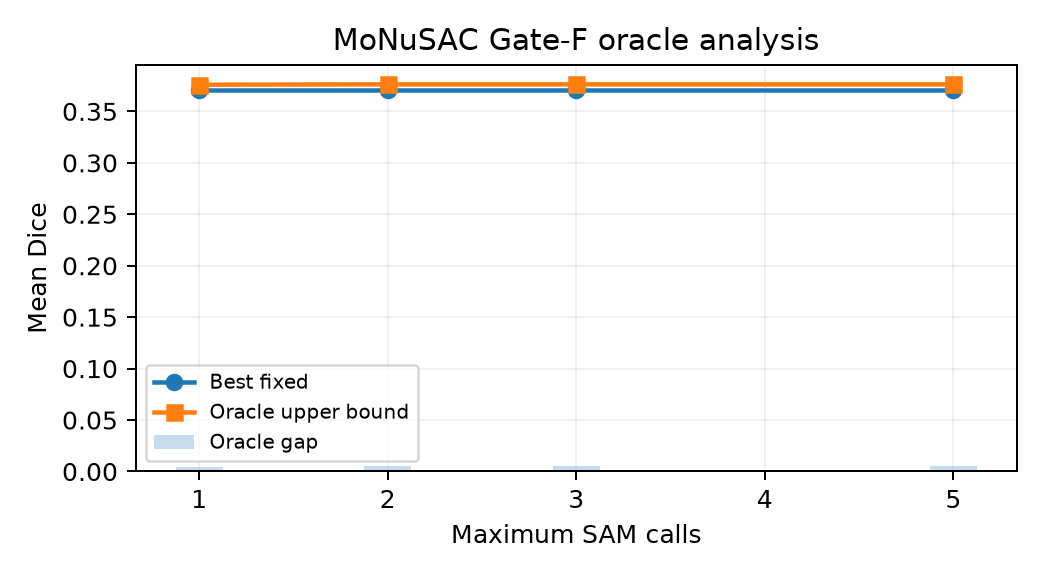
\includegraphics[width=0.47\textwidth]{figures/oracle_pareto.png}
\hfill
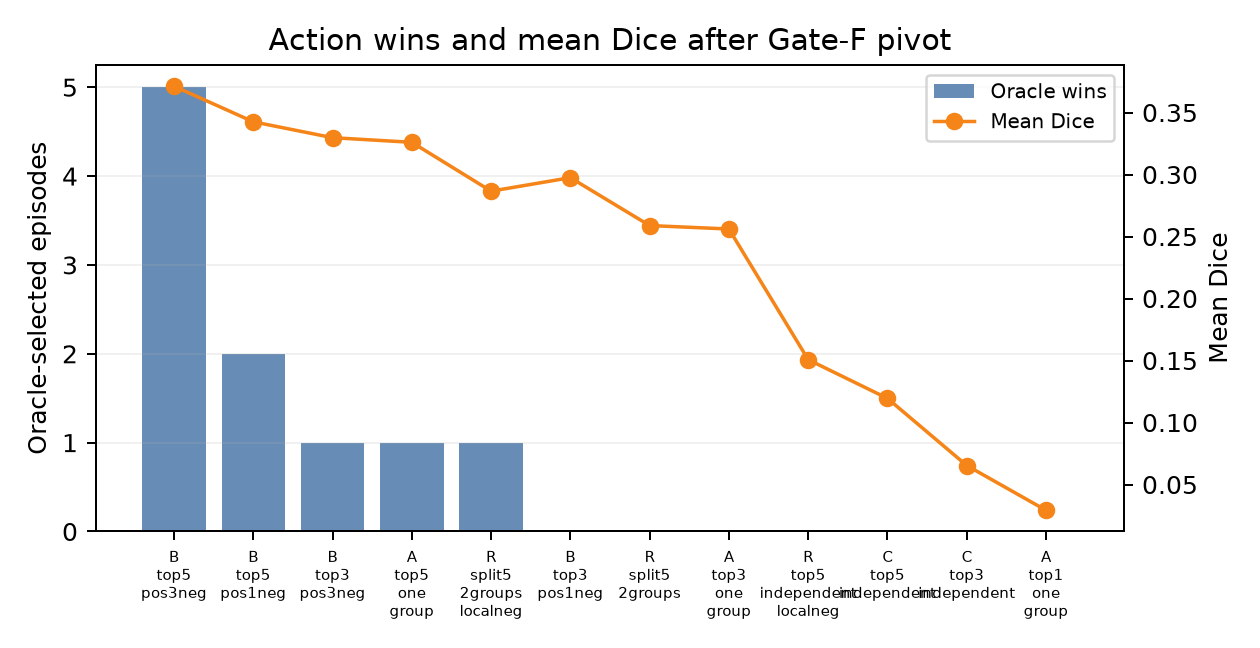
\includegraphics[width=0.47\textwidth]{figures/oracle_action_wins.png}
\caption{Oracle-analysis figures generated from the current MoNuSAC Gate-F pivot artifacts. Left: matched-budget best-fixed and oracle Dice. Right: oracle action counts and mean Dice by action. These are analysis upper bounds, not deployable method outputs.}
\label{fig:oracle-analysis}
\end{figure*}
% Auto-generated from real oracle-analysis artifacts.
\begin{table*}[t]
\centering
\small
\caption{Gate-F pivot status from real pilot artifacts. Oracle columns are analysis upper bounds, not deployable method outputs; no privileged-input row is included.}
\label{tab:oracle-pivot}
\begin{tabular}{llrrrrl}
\toprule
Dataset & Decision & Episodes & Actions & Fixed Dice & Oracle Dice & Claim \\
\midrule
MoNuSAC & Pivot oracle analysis & 10 & 12 & 0.371 & 0.376 & Oracle analysis only \\
GlaS & Pending insufficient episodes & 1 & N/A & 0.718 & 0.718 & Extension smoke only \\
\bottomrule
\end{tabular}
\end{table*}

% Auto-generated from reports/fixed_oracle_analysis/action_summary.csv.
\begin{table*}[t]
\centering
\small
\caption{MoNuSAC action-oracle summary after the Gate-F pivot. Oracle wins are post-hoc analysis labels, not deployable method selections; no privileged-input row is included.}
\label{tab:action-summary}
\begin{tabular}{lrrr}
\toprule
Action & Dice & Calls & Oracle wins \\
\midrule
B\_top5\_pos3neg & 0.371 & 1.00 & 5 \\
B\_top5\_pos1neg & 0.343 & 1.00 & 2 \\
B\_top3\_pos3neg & 0.330 & 1.00 & 1 \\
A\_top5\_one\_group & 0.326 & 1.00 & 1 \\
B\_top3\_pos1neg & 0.297 & 1.00 & 0 \\
R\_split5\_2groups\_localneg & 0.287 & 2.00 & 1 \\
R\_split5\_2groups & 0.259 & 2.00 & 0 \\
A\_top3\_one\_group & 0.256 & 1.00 & 0 \\
R\_top5\_independent\_localneg & 0.151 & 5.00 & 0 \\
C\_top5\_independent & 0.119 & 5.00 & 0 \\
C\_top3\_independent & 0.065 & 3.00 & 0 \\
A\_top1\_one\_group & 0.029 & 1.00 & 0 \\
\bottomrule
\end{tabular}
\end{table*}

Representation diagnostics remain \RepresentationAnalysisClaim{}: the mean top-two action margin is \RepresentationAnalysisTopTwoMargin{}, with near-tie fraction \RepresentationAnalysisNearTieFraction{}.
% Auto-generated from reports/representation_analysis/representation_summary.json.
\begin{table*}[t]
\centering
\small
\caption{Representation diagnostics for the Gate-F pivot. The row uses fixed artifact diagnostics only; no privileged-input row is included.}
\label{tab:representation-pivot}
\begin{tabular}{lrrrrr}
\toprule
Status & Top-2 margin & Near ties & Point precision & Component coverage & Precision-regret $r$ \\
\midrule
Pivot representation analysis & 0.020 & 0.400 & 0.520 & 0.052 & -0.214 \\
\bottomrule
\end{tabular}
\end{table*}

\subsection{Gate-F Interpretation}
The main numerical result is the absence of enough oracle headroom. The measured Dice gap is below the predeclared 0.010 threshold, and the AJI gap is also below the auxiliary threshold used for the pivot decision. The top oracle action fraction is 0.5, so the result is not a trivial one-action dominance story, but the available headroom is still too small to justify policy learning. The deterministic promotion check is also not satisfied, because the current analysis does not prove that one fixed action is a complete deterministic method across the intended domain.

The action summary shows that the best fixed rule is a positive-negative prompt-set action. However, oracle wins are post-hoc labels. They should be read as a diagnostic of action-bank behavior, not as method outputs. Matched-budget analysis is especially important here: the oracle advantage cannot be written as an efficiency result, and higher-call actions do not create a clear quality gain in the current pilot.

\subsection{Failure Diagnostics}
The post-failure audit records three complementary diagnostics. Candidate coverage is low: mean component coverage at the maximum pilot pool is about 0.052, even though point precision at the same pool is above the random baseline. Action proposals are not all identical: the mean top-two Dice margin is about 0.020, and 40\% of episodes are near ties under the configured tolerance. SAM sensitivity does not favor more calls: the best high-call action is lower than the best one-call action by about 0.021 Dice in the diagnostic artifact. Together these facts support a cautious interpretation: the current evidence exposes limitations in candidates and grouping sensitivity, but it does not produce an actionable oracle gap for a MoNuSAC policy.

\subsection{Statistics}
The paired sign-flip diagnostic on query-level deltas records one win, one tie, and zero losses for oracle versus best fixed under the current tie threshold. The two-sided sign-flip $p$ value is 0.5, and patient-cluster bootstrap is marked pending because only one patient cluster is available. These statistics are included to prevent over-reading the mean gap. A future formal study would need enough independent patient or case clusters before confidence intervals could support a stronger result.

\subsection{External Readiness}
GlaS is the first registered external morphology-shift path, but the present evidence is a one-episode smoke only. Its Gate F status is pending because the gate minimum is ten episodes. DDR is ready for infrastructure-only stage-one checks with a binary union of EX, HE, MA, and SE lesion masks, but that stage is not a formal policy task. IDRID remains read-only because previous observations cannot be reused for method selection. CPM-17 is deferred until the missing or incomplete local assets are repaired under an approved protocol. These external records are useful because they define how the project can continue without reopening the failed MoNuSAC policy path.
